\documentclass[letterpaper,11pt,oneside,reqno]{article}

%%%%%%%%%%%%%%%%%%%%%%%%%%%%%%%%%%%%%%%%%%%%%%%%%%%%%%%%%%%%

\usepackage[pdftex,backref=page,colorlinks=true,linkcolor=blue,citecolor=red]{hyperref}
\usepackage[alphabetic,nobysame]{amsrefs}

%%%%%%%%%%%%%%%%%%%%%%%%%%%%%%%%%%%%%%%%%%%%%%%%%%%%%%%%%%%%
%main packages
\usepackage{amsmath,amssymb,amsthm,amsfonts,mathtools}
\usepackage{graphicx,color}
\usepackage{upgreek}
\usepackage[mathscr]{euscript}

%equations
\allowdisplaybreaks
\numberwithin{equation}{section}

%tikz
\usepackage{tikz}
\usetikzlibrary{shapes,arrows,positioning,decorations.markings}

%conveniences
\usepackage{array}
\usepackage{adjustbox}
\usepackage{cleveref}
\usepackage{enumerate}
\usepackage{datetime}
\usepackage{esint}

%paper geometry
\usepackage[DIV=12]{typearea}

%%%%%%%%%%%%%%%%%%%%%%%%%%%%%%%%%%%%%%%%%%%%%%%%%%%%%%%%%%%%
%draft-specific
\synctex=1
% \usepackage{refcheck,comment}

%%%%%%%%%%%%%%%%%%%%%%%%%%%%%%%%%%%%%%%%%%%%%%%%%%%%%%%%%%%%
%this paper specific
\newcommand{\ssp}{\hspace{1pt}}

%%%%%%%%%%%%%%%%%%%%%%%%%%%%%%%%%%%%%%%%%%%%%%%%%%%%%%%%%%%%
\newtheorem{proposition}{Proposition}[section]
\newtheorem{lemma}[proposition]{Lemma}
\newtheorem{corollary}[proposition]{Corollary}
\newtheorem{theorem}[proposition]{Theorem}
%%%%%%%%%%%%%%%%%%%%%%%%%%%%%%%%%%%%%%%%%%%%%%%%%%%%%%%%%%%%
\theoremstyle{definition}
\newtheorem{definition}[proposition]{Definition}
\newtheorem{remark}[proposition]{Remark}
%%%%%%%%%%%%%%%%%%%%%%%%%%%%%%%%%%%%%%%%%%%%%%%%%%%%%%%%%%%%

\newenvironment{lnotes}{\section*{Notes for the lecturer}}{}

% \excludecomment{lnotes}

\begin{document}
\title{Lectures on Random Matrices
(Spring 2025)
\\Lecture 6: Double contour integral kernel. Steepest descent and local statistics}

\date{Wednesday, February 19, 2025\footnote{\href{https://lpetrov.cc/rmt25/}{\texttt{Course webpage}}
$\bullet$ \href{https://lpetrov.cc/simulations/model/random-matrices/}{\texttt{Live simulations}}
$\bullet$ \href{https://lpetrov.cc/rmt25/rmt25-notes/rmt2025-l06.tex}{\texttt{TeX Source}}
$\bullet$
Updated at \currenttime, \today}}

\author{Leonid Petrov}

\maketitle
\tableofcontents

\begin{lnotes}

\begin{itemize}
	\item GUE det structure

	\item Formulate Cauchy--Binet and Andreief

	\item Recall that $\rho_n=P_n$ and it is
	$\left( \det[\psi_i(x_j)]_{n\times n} \right)^2$, then reproduce the proofs here.

	\item Recall the Christoffel--Darboux formula:
	\begin{equation*}
		K_n(x,y)=\frac{e^{-\frac{x^2+y^2}{4}}}{\sqrt{2\pi}
		h_{n-1}}\,\frac{p_n(x)p_{n-1}(y)-p_{n-1}(x)p_n(y)}{x-y},
	\end{equation*}
	here $h_{n-1}=\sqrt{2\pi}(n-1)!$.
\end{itemize}

\end{lnotes}

\section{Recap: Determinantal structure of the GUE}

Last time, we proved the following result:
\begin{theorem}
\label{thm:determinantal_GUE}
The GUE correlation functions are given by
\[
\rho_k(x_1,\dots,x_k)=\det\Bigl[K_n(x_i,x_j)\Bigr]_{i,j=1}^k,
\]
with the correlation kernel
\[
K_n(x,y)=\sum_{j=0}^{n-1}\psi_j(x)\psi_j(y).
\]
Here
\begin{equation*}
	\psi_j(x)=\frac{1}{\sqrt{h_j}}\ssp p_j(x)\,e^{-x^2/4},
\end{equation*}
where \(p_j(x)\) are the monic Hermite polynomials, and \(h_j\) are the normalization constants so that
$\psi_j(x)$ are orthonormal in $L^2(\mathbb{R})$.
\end{theorem}

For this theorem, we need Cauchy--Binet summation formula
and Andreief identity (which is essentially the same as Cauchy--Binet, but when summation is
replaced by integration). Having these, we can write
\begin{align*}
	\rho_k(x_1,\dots,x_k)&=\frac{n!}{(n-k)!}\int_{\mathbb{R}^{n-k}} p(x_1,\dots,x_n) \,dx_{k+1}\cdots dx_n
	\\
	&=
	\frac{1}{(n-k)!\,\widehat{Z}_{n,2}}
	\sum_{\substack{\sigma,\tau\in S_n\\
	\sigma(k+1)=\tau(k+1),\ldots,\sigma(n)=\tau(n) }} \operatorname{sgn}(\sigma)\operatorname{sgn}(\tau)
	\prod_{i=1}^k \psi_{\sigma(i)-1}(x_i)\psi_{\tau(i)-1}(x_i)
	\\
	&=
	\mathrm{const}_n\sum_{I\subseteq [n],\,|I|=k}
	\sum_{\sigma',\tau'\in S(I)}
	\operatorname{sgn}(\sigma')\operatorname{sgn}(\tau')
	\prod_{i=1}^k \psi_{\sigma'(i)-1}(x_i)\psi_{\tau'(i)-1}(x_i)
	\\
	&=
	\mathrm{const}_n\sum_{I\subseteq [n],\,|I|=k}
	\det\left[ \psi_{i_\alpha}(x_j) \right]_{\alpha,j=1}^k
	\det\left[ \psi_{i_\alpha}(x_j) \right]_{\alpha,j=1}^k,
\end{align*}
where \(I=\{i_1,\ldots,i_k\}\) is a subset of \([n]\) of size \(k\), and \(S(I)\) is the set of permutations of \(I\).
The last sum of products of two determinants is
written by the Cauchy--Binet formula as
\begin{equation*}
	\mathrm{const}_n\cdot \det\left[ \sum_{j=0}^{n-1}\psi_j(x_\alpha)\psi_j(x_\beta) \right]_{\alpha,\beta=1}^k,
\end{equation*}
and finally the constant is equal to $1$ by Andreief identity.


%%%%%%%%%%%%%%%%%%%%%%%%%%%%%%%%%%%%%%%%%%%%%%%%%%%%%%%%%%%%
\section{Double Contour Integral Representation for the GUE Kernel}
\label{sec:double-contour}

\subsection{One contour integral representation for Hermite polynomials}

Recall that the GUE kernel is defined by
\[
K_N(x,y)=\sum_{n=0}^{N-1}\psi_n(x)\psi_n(y),
\]
with the orthonormal functions
\[
\psi_n(x)=\frac{1}{\sqrt{h_n}}\,p_n(x)\,e^{-x^2/4},
\]
where the (monic, probabilists') Hermite polynomials are given by
\begin{equation}
\label{eq:hermite_def}
	p_n(x)=(-1)^n e^{x^2/2}\frac{d^n}{dx^n}\,e^{-x^2/2}.
\end{equation}
Note that the monic Hermite polynomials are uniquely defined by the
orthogonality property. We are not proving \eqref{eq:hermite_def} here,
it is an exercise.
\begin{lemma}[Generator function for Hermite polynomials]
	\label{lem:hermite_gen}
	We have
	\[
		\exp\Bigl(xt-\frac{t^2}{2}\Bigr)=\sum_{n\ge0}p_n(x)\frac{t^n}{n!}.
	\]
	The series converges for all \(t\) since the left-hand side is an entire function of \(t\).
\end{lemma}
\begin{proof}
Write the generating function as
\[
	\sum_{n\ge0}p_n(x)\frac{t^n}{n!}
	=\sum_{n\ge0}\frac{(-1)^n t^n}{n!}\,e^{x^2/2}\frac{d^n}{dx^n}\,e^{-x^2/2}.
\]
Since the factor \(e^{x^2/2}\) does not depend on \(n\), we can factor it out:
\[
	\sum_{n\ge0}p_n(x)\frac{t^n}{n!}= e^{x^2/2}\sum_{n\ge0}\frac{(-t)^n}{n!}\frac{d^n}{dx^n}\,e^{-x^2/2}.
\]
Now, recall Taylor's theorem: for any holomorphic function \(f\) we have
\[
	f(x-t)=\sum_{n\ge0}\frac{(-t)^n}{n!}f^{(n)}(x).
\]
Applying this with \(f(x)=e^{-x^2/2}\), we deduce that
\[
	\sum_{n\ge0}\frac{(-t)^n}{n!}\frac{d^n}{dx^n}\,e^{-x^2/2}= e^{-(x-t)^2/2}.
\]
Thus, our generating function becomes
\[
	\sum_{n\ge0}p_n(x)\frac{t^n}{n!} = e^{x^2/2}\, e^{-(x-t)^2/2},
\]
as desired.
\end{proof}


By Cauchy's integral formula we can write using \Cref{lem:hermite_gen}:
\begin{equation}
\label{eq:pn-formula}
p_n(x)=\frac{n!}{2\pi i}\oint_C\frac{\exp\Bigl(xt-\frac{t^2}{2}\Bigr)}{t^{n+1}}\,dt,
\end{equation}
where the contour \(C\) is a simple closed curve encircling the origin.
Indeed, here we use the complex analysis property
\begin{equation*}
	\frac{1}{2\pi i}\oint_C \frac{1}{z^{k+1}}\ssp dz=\begin{cases}
		1,&\text{ if }k=0,\\
		0,&\text{ if }k\neq0,
	\end{cases}
\end{equation*}
so \eqref{eq:pn-formula} is simply a complex analysis version of the
operation of extracting the coefficient of \(t^n\) in the Taylor expansion.

Therefore,
\begin{equation*}
	\psi_n(x)=\frac{1}{\sqrt{h_n}}\,p_n(x)\,e^{-x^2/4}=
	\frac{e^{-x^2/4}}{\sqrt{h_n}}\frac{n!}{2\pi i}\oint_C\frac{\exp\Bigl(xt-\frac{t^2}{2}\Bigr)}{t^{n+1}}\,dt.
\end{equation*}

\subsection{Another contour integral representation for Hermite polynomials}

We start with the Fourier transform identity
\[
\int_{-\infty}^{\infty} \exp\Bigl(-\frac{t^2}{2} + i\,t\,x\Bigr)\,dt
=\sqrt{2\pi}\,e^{-x^2/2}.
\]
Differentiating both sides \(n\) times with respect to \(x\) yields
\[
\frac{d^n}{dx^n}\Bigl(e^{-x^2/2}\Bigr)
=\frac{1}{\sqrt{2\pi}}\int_{-\infty}^{\infty} (i\,t)^n\,e^{-t^2/2+ i\,t\,x}\,dt.
\]
Recalling the definition
\[
p_n(x)=(-1)^n\,e^{x^2/2}\,\frac{d^n}{dx^n}\Bigl(e^{-x^2/2}\Bigr),
\]
we obtain
\[
p_n(x)=\frac{(-1)^n\,e^{x^2/2}}{\sqrt{2\pi}}\int_{-\infty}^{\infty}(i\,t)^n\,e^{-t^2/2+ i\,t\,x}\,dt.
\]

Next, perform the change of variable
\[
s=i\,t,\quad\text{so that}\quad t=-i\,s,\quad dt=-i\,ds.
\]
Under this substitution the factors transform as follows:
\[
(i\,t)^n = s^n,
\]
and the exponent becomes
\[
-\frac{t^2}{2}+ i\,t\,x
= -\frac{(-i\,s)^2}{2}+ i\,(-i\,s)\,x
= \frac{s^2}{2}+ s\,x.
\]
Thus, the integral transforms into
\[
\int_{-\infty}^{\infty}(i\,t)^n\,e^{-t^2/2+ i\,t\,x}\,dt
= -i \int_{-i\infty}^{i\infty} s^n\,e^{s^2/2+ s\,x}\,ds.
\]
Substituting back we have
\[
p_n(x)=\frac{(-1)^n\,e^{x^2/2}}{\sqrt{2\pi}}\;(-i)
\int_{-i\infty}^{i\infty} s^n\,e^{s^2/2+ s\,x}\,ds.
\]
That is,
\[
p_n(x)=\frac{i\,(-1)^{n+1}\,e^{x^2/2}}{\sqrt{2\pi}}
\int_{-i\infty}^{i\infty} s^n\,e^{s^2/2+ s\,x}\,ds.
\]
Finally, change the sign of $s$, and we get:
\[
p_n(x)=\frac{i\,e^{x^2/2}}{\sqrt{2\pi}}
\int_{-i\infty}^{i\infty} s^n\,e^{s^2/2- s\,x}\,ds.
\]
Therefore,
\[
\psi_n(x)=\frac{i\,e^{x^2/4}}{\sqrt{2\pi\,h_n}}
\int_{-i\infty}^{i\infty} s^n\,e^{s^2/2- s\,x}\,ds.
\]

\subsection{Normalization of Hermite polynomials}

\begin{lemma}
	\label{lem:hermite_norm}
	We have
	\begin{equation*}
		h_n=\int_{-\infty}^{\infty} p_n(x)^2\,e^{-x^2/2}\,dx=n!\sqrt{2\pi}.
	\end{equation*}
\end{lemma}
\begin{proof}
Multiply the generating function
\[
	\exp\Bigl(xt-\frac{t^2}{2}\Bigr)=\sum_{n\ge0}p_n(x)\frac{t^n}{n!}
\]
with a second copy (with parameter \(s\)):
\[
	\exp\Bigl(xs-\frac{s^2}{2}\Bigr)=\sum_{m\ge0}p_m(x)\frac{s^m}{m!}.
\]
Then,
\[
	\exp\Bigl(xt-\frac{t^2}{2}\Bigr)\exp\Bigl(xs-\frac{s^2}{2}\Bigr)
	=\sum_{n,m\ge0}p_n(x)p_m(x)\frac{t^n s^m}{n!m!}.
\]
Integrate both sides against \(e^{-x^2/2}\,dx\). Using the orthogonality
\[
	\int_{-\infty}^{\infty}p_n(x)p_m(x)e^{-x^2/2}dx=h_n\delta_{nm},
\]
the right-hand side becomes
\[
	\sum_{n\ge0}\frac{h_n}{(n!)^2}(ts)^n.
\]
On the left-hand side, we have
\[
	\int_{-\infty}^{\infty}e^{-x^2/2}\exp\Bigl(x(t+s)-\frac{t^2+s^2}{2}\Bigr)dx.
\]
Completing the square in \(x\) or recalling the standard Gaussian integral yields
\[
	\sqrt{2\pi}\exp\Bigl(\frac{(t+s)^2-(t^2+s^2)}{2}\Bigr)
	=\sqrt{2\pi}\exp(ts).
\]
Thus, we obtain
\[
	\sqrt{2\pi}\exp(ts)=\sum_{n\ge0}\frac{h_n}{(n!)^2}(ts)^n.
\]
Expanding the left side as
\[
	\sqrt{2\pi}\sum_{n\ge0}\frac{(ts)^n}{n!},
\]
and comparing coefficients, we conclude that
\[
	\frac{h_n}{(n!)^2}=\frac{\sqrt{2\pi}}{n!}\quad\Longrightarrow\quad h_n=n!\sqrt{2\pi}.
\]
This completes the proof.
\end{proof}

\subsection{Double contour integral representation for the GUE kernel}

We can sum up the kernel (essentially, this is
another proof of the Christoffel--Darboux formula):
\begin{equation}\begin{split}
	K_n(x,y)&=
	\sum_{k=0}^{n-1}\psi_k(x)\psi_k(y)
	\\&=
	\frac{e^{\frac{x^2-y^2}{4}}}{(2\pi)^2}
	\oint_C dt\int_{-i\infty}^{i\infty}ds\ssp
	\exp\left\{ -\frac{t^2}{2}+xt+\frac{s^2}{2}-ys \right\}
	\underbrace{\sum_{k=0}^{n-1}
	s^k t^{-k-1}}_{\frac{1-(s/t)^n}{t-s}}.
\end{split}\label{eq:K_n_sum}\end{equation}
Here we used the two contour integral representations for Hermite polynomials,
and the explicit norm (\Cref{lem:hermite_norm}).
At this point, the $t$ contour is a small circle around $0$, and
the $s$ contour is a vertical line in the complex plane.
Their mutual position can be arbitrary at this point --- the $s$ contour
goes along the imaginary line.
Indeed, the fraction
$\frac{1-(s/t)^n}{t-s}$ does not have a singularity at $s=t$ due to the
cancellation.

Let us now move the $s$ contour to be to the left of the $t$ contour,
as in \Cref{fig:contours}.
On the new contours, we have $|s|>|t|$.
Now we can add the summands $s^k t^{-k-1}$
for all $k\le -1$
into the sum in
\eqref{eq:K_n_sum}.
Indeed, for $|s|>|t|$, the series in $k$ converges, while the
summand $s^kt^{-k-1}$ has zero residue at $0$ and thus adding the
summands does not change the value of the integral.

\begin{figure}[htpb]
	\centering
	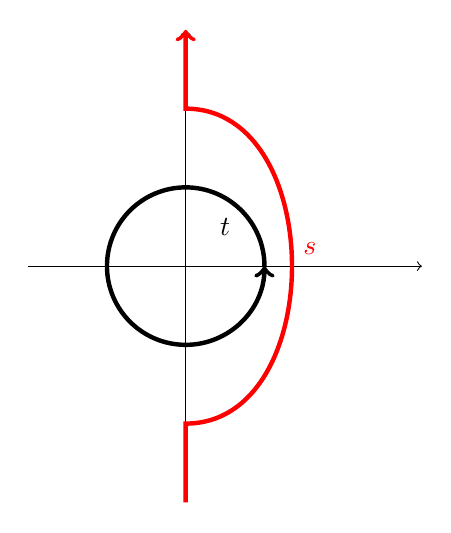
\begin{tikzpicture}[scale=1]
		% Draw coordinate axes
		\draw[->] (-2,0) -- (3,0);
		\draw[->] (0,-3) -- (0,3);

		% t contour: unit circle, counterclockwise
		\draw[ultra thick,->] (1,0) arc (0:360:1);
		% Place the t label near the contour (at 45° outside the circle)
		\coordinate (TLabel) at (.5,.5);
		\node at (TLabel) {\(t\)};

		% s contour: vertical line (imaginary axis) with a detour near the origin
		% It starts at (0,-3), goes vertically to (0,-2), then detours to (0,2)
		% via a Bézier curve (pushed to the right), and finally resumes vertically to (0,3).
		\draw[ultra thick,->,red]
			(0,-3)
			-- (0,-2)
			.. controls (1.8,-2) and (1.8,2) .. node[midway, above right] {\(s\)} (0,2)
			-- (0,3);
	\end{tikzpicture}
	\caption{Integration contours for the GUE kernel \eqref{eq:K_n_GUE_kernel}.}
	\label{fig:contours}
\end{figure}

With this extension of the sum, formula \eqref{eq:K_n_sum} becomes
\begin{equation}
	\label{eq:K_n_GUE_kernel}
	K_n(x,y)=\frac{e^{(y^2-x^2)/4}}{(2\pi)^2}
	\oint_C dt\int_{-i\infty}^{i\infty}ds\ssp
	\frac{\exp\left\{ \frac{s^2}{2}-sy-\frac{t^2}{2}+tx \right\}}{s-t}\left( \frac{s}{t} \right)^n
	.
\end{equation}

\begin{remark}
	The $s$ contour passes to the right of the $t$ contour, but it might as well
	pass to the left of it. Indeed, one can deform the $s$ contour to the left
	while picking the residue at $s=t$:
	\begin{equation*}
		2\pi i\ssp
		\operatorname{Res}\limits_{s=t}
		\frac{\exp\left\{ \frac{s^2}{2}-sy-\frac{t^2}{2}+tx \right\}}{s-t}\left( \frac{s}{t} \right)^n
		=-e^{t(x-y)}.
	\end{equation*}
	This function is entire in $t$, and its
	integral over the $t$ contour is zero.
	Therefore, there is no difference where the $s$ contour passes with respect to the $t$ contour.
\end{remark}

\subsection{Conjugation of the kernel}

The kernel $K_n(x,y)$ contains a factor $e^{\frac{y^2-x^2}{4}}=g(x)/g(y)$,
where $g(\cdot)$ is a nonvanishing function. This factor can be safely removed, since
in all determinants
$\det[K_n(x_i,x_j)]_{i,j=1}^k$
representing the correlation functions, the
conjugation factors $g(x_i)/g(x_j)$ do not affect the value of the determinant.
Thus, we can and will deal with the correlation kernel
\begin{equation}
	\label{eq:K_n_conjugated}
	K_n(x,y)=\frac{1}{(2\pi)^2}
	\oint_C dt\int_{-i\infty}^{i\infty}ds\ssp
	\frac{\exp\left\{ \frac{s^2}{2}-sy-\frac{t^2}{2}+tx \right\}}{s-t}\left( \frac{s}{t} \right)^n
	,
\end{equation}
and will use the same notation for it.
Throughout the asymptotic analysis in \Cref{sec:steepest-descent-GUE} below,
other conjugation factors may appear, but we can similarly
remove them.

\subsection{Extensions}

Many other versions of the GUE / unitary invariant ensembles admit determinantal structure:
\begin{enumerate}
	\item The GUE corners process \cite{johansson2006eigenvalues}
    \item The Dyson Brownian motion (e.g., add a GUE to a diagonal matrix)
			\cite{nagao1998multilevel}
		\item GUE corners plus a fixed matrix \cite{Ferrari2014PerturbedGUE}
    \item Corners invariant ensembles with fixed eigenvalues $UDU^\dagger$, where $D$ is a fixed diagonal matrix and $U$ is Haar distributed
			on the unitary group \cite{Metcalfe2011GT}
	\end{enumerate}

We will discuss the corners process structure
in the next
\href{https://lpetrov.cc/rmt25/rmt25-notes/rmt2025-l07.pdf}{Lecture 7}.

%%%%%%%%%%%%%%%%%%%%%%%%%%%%%%%%%%%%%%%%%%%%%%%%%%%%%%%%%%%%

%%%%%%%%%%%%%%%%%%%%%%%%%%%%%%%%%%%%%%%%%%%%%%%%%%%%%%%%%%%%
\section{Steepest descent --- generalities for single integrals}
%%%%%%%%%%%%%%%%%%%%%%%%%%%%%%%%%%%%%%%%%%%%%%%%%%%%%%%%%%%%

\subsection{Setup}

In many problems arising in random matrix theory—as well as in asymptotic analysis more generally—it is necessary to evaluate integrals of the form
\begin{equation}
	\label{eq:general-integral}
	I(\Lambda)=\int_{\gamma} e^{\Lambda f(z)}\ssp \phi(z)\,dz,
\end{equation}
where
\begin{itemize}
	\item $\Lambda>0$ is a large parameter,
	\item $f(z)$ and $\phi(z)$ are holomorphic functions in a neighborhood of the contour $\gamma\subset\mathbb{C}$,
	\item and the contour $\gamma$ is chosen in such a way that the integral converges.
\end{itemize}
The \emph{method of steepest descent} (also known as the \emph{saddle point method}) provides a systematic procedure for obtaining the asymptotic behavior of $I(\Lambda)$ as $\Lambda\to+\infty$.

The key observation is that for large $\Lambda$, the
exponential term $e^{\Lambda f(z)}$ is highly oscillatory or
decaying, so that the main contributions to the integral
come from small neighborhoods of points where the real part
of $f(z)$ is maximal.
Moreover, since we can deform the integration contour $\gamma$
to pick points where $\operatorname{Re}f(z)$ is even bigger, it makes sense to find
points \emph{not only on the original contour}
where $\operatorname{Re}f(z)$ is maximal.
Such \emph{critical} (or \emph{saddle}) points are
found from the equation with the complex derivative:
\begin{equation*}
	f'(z)=0
\end{equation*}
Indeed, since $\operatorname{Re}f(z)$
is harmonic and $f(z)$ satisfies the Cauchy--Riemann equations,
the condition $f'(z)=0$ is equivalent to the condition that $\operatorname{Re}f(z)$
has zero gradient. Moreover, by harmonicity, all critical points of
$\operatorname{Re}f(z)$ are saddle-like.

Once the saddle points are identified, one deforms the
contour $\gamma$ to $\Gamma$ so that $\Gamma$ passes
through the saddle point(s)
with the maximal value of $\operatorname{Re}f(z)$, and, moreover,
such that on the rest of the new contour $\Gamma$ the
real part of $f(z)$ is strictly less than the value(s) at the saddle point(s).
The decrease of $\operatorname{Re}f(z)$ along $\Gamma$ may be ensured
if one picks $\Gamma$ to be \emph{steepest descent} for $\operatorname{Re}f(z)$.
By holomorphicity of $f(z)$, the steepest descent
of $\operatorname{Re}$ is equivalent to the condition that
the imaginary part of $f(z)$ is constant along $\Gamma$.

\begin{remark}
	\label{rem:steepest-descent}
	In practical applications, one does not
	need $\Gamma$ to be fully steepest descent (it is usually hard to control).
	One can either choose $\Gamma$ to be steepest descent
	in a neighborhood of the critical point and estimate the real part outside,
	or simply estimate the change of $\operatorname{Re}f(z)$ directly along a given contour.
\end{remark}

\begin{remark}
	\label{rem:residues}
	The function $\phi(z)$ might not be holomorphic, and might have poles. The
	deformation of the contour from $\gamma$ to $\Gamma$ might pick residues
	at these poles. These residues can be harmless (easy to account for) or
	not (hard to account for; or affect the asymptotics of the integral),
	and one has to be careful with the contour deformation.
\end{remark}

Despite the caveats in \Cref{rem:steepest-descent,rem:residues},
in what follows in this section we will discuss the
easiest case of steepest descent analysis.
We also assume that there is only one saddle point $z_0$
to take care of.

%%%%%%%%%%%%%%%%%%%%%%%%%%%%%%%%%%%%%%%%%%%%%%%%%%%%%%%%%%%%
\subsection{Saddle points and steepest descent paths}
%%%%%%%%%%%%%%%%%%%%%%%%%%%%%%%%%%%%%%%%%%%%%%%%%%%%%%%%%%%%

\begin{definition}[Saddle point]
	A point $z_0\in\mathbb{C}$ is called a \emph{saddle point} of $f(z)$ if
	\[
		f'(z_0)=0.
	\]
	We shall assume in what follows that at every saddle point under consideration the second derivative satisfies
	\[
		f''(z_0)\neq 0.
	\]
\end{definition}

\begin{definition}[Steepest descent path]
	Let $z_0$ be a saddle point of $f(z)$. A curve $\Gamma\subset\mathbb{C}$ passing through $z_0$ is called a \emph{steepest descent path} for $f(z)$ if along $\Gamma$ the imaginary part of $f(z)$ is constant (i.e.,
	\(
		\operatorname{Im}\bigl(f(z)\bigr)=\operatorname{Im}\bigl(f(z_0)\bigr)
	\)
	for all $z\in\Gamma$), which implies that the real part
	$\operatorname{Re}\bigl(f(z)\bigr)$ decreases away from
	$z_0$.
\end{definition}

In a neighborhood of a saddle point $z_0$,
\[
	z=z_0+w,
	\qquad
	f(z)=f(z_0)+\frac{1}{2}f''(z_0)w^2 + O(w^3).
\]
If we denote
\[
	f''(z_0)=|f''(z_0)|e^{i\theta_0},
\]
then writing $w=r\,e^{i\varphi}$, we obtain
\[
	f(z)=f(z_0)+\frac{1}{2}|f''(z_0)|r^2e^{i(2\varphi+\theta_0)}+O(r^3).
\]
For the imaginary part to remain constant in a neighborhood
of $z_0$, and, moreover,
for the phase of the quadratic term to be $\pi$ modulo $2\pi$, one must choose $\varphi$ so that
\begin{equation}
	\label{eq:steepest-descent-direction}
	2\varphi+\theta_0=\pi \quad (\operatorname{mod}\,2\pi).
\end{equation}
We need the phase $\pi$ so that the exponent is negative, for the integral to converge.

There are two directions satisfying \eqref{eq:steepest-descent-direction}
through $z_0$, and we use both of them for our contour $\Gamma$.
Along these directions, one finds that
\[
	\operatorname{Re}\bigl(f(z)\bigr)=\operatorname{Re}\bigl(f(z_0)\bigr)-\frac{1}{2}|f''(z_0)|r^2+O(r^3),
\]
so that $\operatorname{Re}(f(z))$ is maximal at $z=z_0$ and decays quadratically as one moves away from $z_0$ along the steepest descent paths.

%%%%%%%%%%%%%%%%%%%%%%%%%%%%%%%%%%%%%%%%%%%%%%%%%%%%%%%%%%%%
\subsection{Local asymptotic evaluation near a saddle point}
%%%%%%%%%%%%%%%%%%%%%%%%%%%%%%%%%%%%%%%%%%%%%%%%%%%%%%%%%%%%

Assume now that the contour $\gamma$ in \eqref{eq:general-integral} has been deformed so that it passes through a saddle point $z_0$ along a steepest descent path. In a small neighborhood of $z_0$, we write
\[
	z=z_0+w,
\]
so the local contribution of a neighborhood of $z_0$ to the integral is
\begin{equation}
	\label{eq:local-contribution}
	I_{z_0}(\Lambda)=e^{\Lambda f(z_0)}\phi(z_0)
	\int_{-\infty}^{\infty} e^{\Lambda\frac{1}{2}f''(z_0)w^2}\,dw
	\Bigl(1+O\Bigl(\frac{1}{\Lambda}\Bigr)\Bigr).
\end{equation}
Here the integration is taken along the steepest descent direction, so that the quadratic term in the exponent is real and negative. (That is, by the choice \eqref{eq:steepest-descent-direction}, we have $\operatorname{Re}\bigl(f''(z_0)w^2\bigr)=-|f''(z_0)|r^2$.) Then the Gaussian integral evaluates to
\[
	\int_{-\infty}^{\infty} e^{-\Lambda\frac{|f''(z_0)|}{2}r^2}\,dr
	=\sqrt{\frac{2\pi}{\Lambda |f''(z_0)|}}.
\]
Hence, we
arrive at the following fundamental result.

\begin{theorem}[Local asymptotics via steepest descent]
	\label{thm:steepest-descent}
	Let $z_0$ be a saddle point of $f(z)$ with $f'(z_0)=0$ and $f''(z_0)\neq 0$, and assume that $\phi(z)$ is holomorphic in a neighborhood of $z_0$. Then, as $\Lambda\to+\infty$, the contribution of a small neighborhood of $z_0$ to the integral \eqref{eq:general-integral} is given by
	\begin{equation}
		\label{eq:local-asymptotics}
		I_{z_0}(\Lambda)
		\sim e^{\Lambda f(z_0)}\ssp \phi(z_0)
		\sqrt{\frac{2\pi}{\Lambda\,|f''(z_0)|}},\qquad \Lambda\to+\infty.
	\end{equation}
	Moreover, the behavior \eqref{eq:local-asymptotics}
	captures the full asymptotic behavior of the
	integral \eqref{eq:general-integral}
	as long as on the new contour $\Gamma$,
	the real part of $f(z)$ is maximized at $z_0$ and is separated
	from $\operatorname{Re}f(z_0)$ everywhere else on $\Gamma$ outside of a
	small neighborhood of $z_0$.
\end{theorem}

Under appropriate assumptions (typically, if $f$ and $\phi$ are holomorphic on a neighborhood that can be reached by the deformed contour and if the contributions away from the saddle points are exponentially small), one may show that the error in approximating the full integral by the sum of the local contributions is itself exponentially small relative to the leading order terms. In many cases, the next-order corrections can be computed by carrying the expansion in \eqref{eq:local-contribution} to higher order in $w$. (See, e.g., \cite{olver1974asymptotics} for a systematic treatment.)

%%%%%%%%%%%%%%%%%%%%%%%%%%%%%%%%%%%%%%%%%%%%%%%%%%%%%%%%%%%%



\section{Steepest descent for the GUE kernel}
\label{sec:steepest-descent-GUE}

\subsection{Scaling}
\label{sub:scaling}

Let us now consider the GUE kernel
\eqref{eq:K_n_conjugated},
\begin{equation*}
	K_n(x,y)=\frac{1}{(2\pi)^2}
	\oint_C dt\int_{-i\infty}^{i\infty}ds\ssp
	\frac{\exp\left\{ \frac{s^2}{2}-sy-\frac{t^2}{2}+tx \right\}}{s-t}\left( \frac{s}{t} \right)^n
	,
\end{equation*}
where the integration contours are as in \Cref{fig:contours}.

We know from the Wigner semicircle law
(established for real symmetric matrices with general iid entries in
in \href{https://lpetrov.cc/rmt25/rmt25-notes/rmt2025-l02.pdf}{Lecture 2},
and for the GUE in \href{https://lpetrov.cc/rmt25/rmt25-notes/rmt2025-l04.pdf}{Lecture 4})
that the eigenvalues live on the scare $\sqrt n$. This means that to capture the local asymptotics,
we need to scale
\begin{equation}
	\label{eq:scaling_x-y}
	x=X\sqrt n+\frac{\Delta x}{\sqrt n},\qquad y=Y\sqrt n+\frac{\Delta y}{\sqrt n},\qquad
	\Delta x,\Delta y\in\mathbb{R}.
\end{equation}
Moreover, if $X\ne Y$ (i.e., different global positions), one can check that the kernel
vanishes. In other words, the local behaviors at different global positions are independent.
See Problem~\ref{prob:different-global-positions}.
In what follows, we take $Y=X$.

Let us also make a change of the integration variables:
\begin{equation*}
	t=z\sqrt n,\qquad s=w\sqrt n.
\end{equation*}
The integration contours for $z$ and $w$ look the same as in
\Cref{fig:contours}, up to a rescaling. However, as $0$
and $t=s$
are the only singularities in the integrand, we can deform the $z,w$
contours as we wish, while keeping $|z|<|w|$
and the general shape as in \Cref{fig:contours}.

We thus have:
\begin{multline}
	\label{eq:K_n_scaling}
	K_n(X\sqrt n+\Delta x/\sqrt n,X\sqrt n+\Delta y/\sqrt n)\\=
	\frac{\sqrt n}{(2\pi)^2}
	\oint_C dz\int_{-i\infty}^{i\infty}dw\ssp
	\frac{\exp
		\left\{
			n\left(
				\log w -\log z
				+\frac{w^2}{2}-\frac{z^2}{2}
				+X(z-w)+\frac{z \Delta x-w \Delta y}{n}
			\right)
		\right\}
	}{w-z}.
\end{multline}
\begin{remark}
	\label{rmk:log-harmless}
	The logarithms in the exponent are harmless, since for the
	estimates we only need the real parts of the logarithms,
	and for the main contributions, we will have $z\approx w$, so
	any phases of the logarithms would cancel.
\end{remark}

The asymptotic analysis of double contour integrals like
\eqref{eq:K_n_scaling} in the context of determinantal point processes
was pioneered in \cite[Section~3]{Okounkov2002}.

\subsection{Critical points}
\label{sub:critical-points}

Let us define
\begin{equation*}
	S(z)\coloneqq
	\frac{z^2}{2}+\log z -X z.
\end{equation*}
Then the exponent contains $n \left( S(w)-S(z) \right)$.
According to the steepest descent ideology, we
should deform the integration contours
to pass through the critical point(s) $z_{cr}$ of $S(z)$.
Moreover, the new $w$ contour should maximize the real part of $S(z)$
at $z_{cr}$, and the new $z$ contour should minimize it.
If $S''(z_{cr})\ne 0$, it is possible to locally choose such contours,
they will be perpendicular to each other at $z_{cr}$.

Thus, we need to find the critical points of $S(z)$.
They are found from the quadratic equation:
\begin{equation}
	\label{eq:critical-points}
	S'(z)=z+\frac{1}{z}-X=0,\qquad
	z_{cr}=\frac{X\pm \sqrt{X^2-4}}{2}.
\end{equation}
Depending on whether $|X|<2$, there are three cases.
Unless $|X|=2$, equation \eqref{eq:critical-points} has a single root, and
thus $S''(z_{cr})\ne 0$.
We will consider the three cases in
\Cref{sub:imaginary-critical-points,sub:real-critical-points,sub:double-critical-points}
below.

\subsection{Imaginary critical points: $|X|<2$, ``bulk''}
\label{sub:imaginary-critical-points}

When $|X|<2$, the critical points are complex conjugate.
Denote them by $z_{cr}$ and $\overline{z_{cr}}$.
Since $S(z)$ has real coefficients, we have
\begin{equation*}
	\operatorname{Re}S(z_{cr})=\operatorname{Re}S(\overline{z_{cr}}).
\end{equation*}
Thus, we need to consider the contribution from both points.
For simplicity of the computations, let us consider only the case $X=0$.
See Problem~\ref{prob:imaginary-critical-points}.
We have
\begin{equation*}
	z_{cr}=i,\qquad
	S''(z_{cr})=2.
\end{equation*}
The behavior of $\operatorname{Re}S(z)$ on the complex plane
can be illustrated by a 3D plot or by a region plot of the regions
where $\operatorname{Re}S(z)-\operatorname{Re}S(z_{cr})$ has constant sign.
See \Cref{fig:ReS_imaginary} for an illustration in the case $X=\frac{1}{2}$.
(We take $X\ne 0$ to break symmetry, for a better intuition.)

\begin{figure}[htpb]
	\centering
	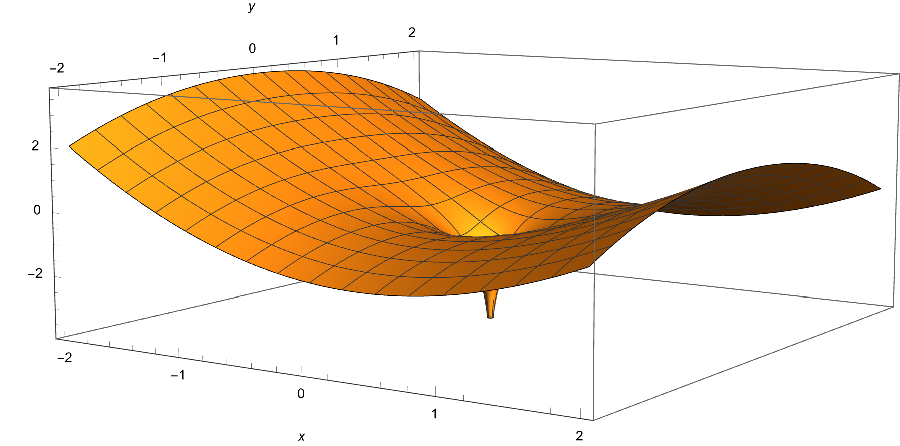
\includegraphics[height=.3\textwidth]{pictures/ReS_imaginary_3D.pdf}
	\qquad
	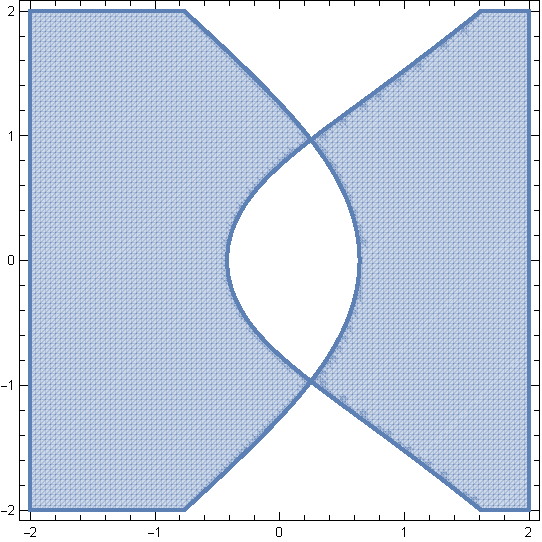
\includegraphics[height=.3\textwidth]{pictures/ReS_imaginary_region.pdf}
	\caption{A 3D plot and a region plot of the
	regions where $\operatorname{Re}S(z)-\operatorname{Re}S(z_{cr})$ is positive
	(highlighted) or negative, in the case $X=\frac{1}{2}$.
	In this case, $z_{cr}\approx 0.25+0.96 i$.}
	\label{fig:ReS_imaginary}
\end{figure}

From the region plot, we see that the new $z$ contour should
pass through the shaded region $\operatorname{Re}S(z)-\operatorname{Re}S(z_{cr})>0$,
and the new $w$ contour should pass through the unshaded region
$\operatorname{Re}S(z)-\operatorname{Re}S(z_{cr})<0$.

Deforming the contours from \Cref{fig:contours} to the new contours
is impossible without passing through the residue at $w=z$.
Moreover, this residue appears only for certain values of $z$. Namely, for $X=0$,
let us first make the $z$ contour to be the positively (counterclockwise) oriented
unit circle.
It passes through the critical points $z_{cr}=i$ and $\overline{z_{cr}}=-i$.
Since the original $w$ contour is to the right of the $z$ contour, we only
encounter the residue when $z$ is in the right half of the circle.

Thus, we can write
\begin{equation}
	\label{eq:K_n_bulk_deformation}
	\oiint_{\textnormal{old contours}}=
	\oiint_{\textnormal{new contours}}
	+
	\int_{-i}^i 2\pi i\ssp \operatorname{Res}\limits_{w=z}\ssp dz,
\end{equation}
where in the single integral, the $z$ contour passes to the right of the origin,
along the right half of the unit circle.

It remains to consider the two integrals in the right-hand side
of \eqref{eq:K_n_bulk_deformation}.
Recall that the correlation functions are
defined relative to a reference measure, and the right object to scale is
\begin{equation*}
	K_n(x,y)dy=\frac{1}{\sqrt n}\ssp d\left( \Delta y \right).
\end{equation*}
The extra factor $n^{-1/2}$
compensates the prefactor $\sqrt n$ in
\eqref{eq:K_n_scaling}.

The single integral takes the form
\begin{equation}
	\label{eq:K_n_bulk_single}
	\frac{-i}{2\pi}
	\int_{-i}^i
	e^{z (\Delta x -\Delta y)}
	\ssp
	dz
	=\frac{\sin\left( \Delta x-\Delta y \right)}{\pi(\Delta x-\Delta y)},
	\qquad \Delta x,\Delta y\in\mathbb{R}.
\end{equation}
\begin{definition}
	\label{def:sine-kernel}
	The \emph{sine kernel} is defined as
	\begin{equation*}
		K_{\mathrm{sine}}(x,y)\coloneqq
		\begin{cases}
			\dfrac{\sin (x-y)}{\pi (x-y)},&\qquad x\ne 0,\\[10pt]
			\dfrac{1}{\pi},&\qquad x=0.
		\end{cases}
	\end{equation*}
	(The value at $x=y$ is defined by continuity.)

	This kernel is translation invariant, and is often
	defined with a single argument, as
	$K_{\mathrm{sine}}(x-y)$.
\end{definition}

The double integral has both contours
in the ``steepest descent'' regime, which means that
the main contribution is
\begin{equation*}
	\mathrm{const}\cdot
	\frac{e^{n\left( \operatorname{Re}S(z_{cr})-\operatorname{Re}S(z_{cr}) \right)}}{\sqrt n}
	\sim \frac{\mathrm{const}}{\sqrt n}.
\end{equation*}
At this rate, the double integral over the new contours
\emph{does not} contribute to the asymptotics of the correlation functions.
Recall that the correlation functions are expressed as finite-dimensional
determinants of the kernel $K_n(x,y)$, and the error $O(n^{-1/2})$ is
negligible in the limit $n\to+\infty$.
This is because the main term comes from the single integral,
which does not vanish.

We have established the following result:
\begin{proposition}[Bulk asymptotics at $X=0$]
	\label{prop:bulk}
	The correlation kernel $K_n$ of the GUE has the following asymptotics
	close to zero as $n\to+\infty$:
	\begin{equation*}
		\lim_{n\to \infty}
		\frac{1}{\sqrt n}
		K_n\left( \frac{\Delta x}{\sqrt n},\frac{\Delta y}{\sqrt n} \right)
		=
		K_{\mathrm{sine}}\left( \Delta x,\Delta y \right),
		\qquad \Delta x,\Delta y\in\mathbb{R}.
	\end{equation*}
	Consequently, the eigenvalues of the GUE converge to the sine process
	determined by the sine kernel (\Cref{def:sine-kernel}),
	in the sense of finite-dimensional distributions.
\end{proposition}

\begin{remark}
	Beyond $X=0$, the local correlations are essentially the same,
	up to rescaling of the real line by a constant factor (depending
	on the semicircle density).
	See Problem~\ref{prob:imaginary-critical-points}.
\end{remark}

\subsection{Real critical points: $|X|>2$, ``large deviations''}
\label{sub:real-critical-points}

For \(X^2>4\), both solutions
\eqref{eq:critical-points}
are real. Let us assume $X>2$, the case \(X<2\) is similar.
For $X>2$, both solutions are positive.
Label these solutions as
\[
	z_+ \;=\;\frac{X + \sqrt{X^2-4}}{2},
	\qquad
	z_- \;=\;\frac{X - \sqrt{X^2-4}}{2},
	\quad
	\text{so that}\quad z_+z_-=1.
\]
A straightforward check reveals that \(z_+\!>\!1\) and \(z_-\!<\!1\) (for \(X>2\)).
Note that $S''(z)=1-z^{-2}$, which is positive for \(z_+>1\) and negative for \(z_-<1\).  Thus, the critical points \(z_+\) and \(z_-\) are a local minimum and a local maximum.
A crucial observation is that
\begin{equation*}
	S(z_+)<S(z_-).
\end{equation*}
One can deform the $z$ integration contour to pass through
$z_-$ and the $w$ contour to pass through $z_+$.
Then, on these contours, one can show that
\begin{equation*}
	\operatorname{Re}S(w)-\operatorname{Re}S(z)<0.
\end{equation*}
According to the steepest descent ideology,
we see that the main exponential behavior of the double contour integral is
\begin{equation}
	\label{eq:Oexp}
	\exp\left\{ n\left(
		\operatorname{Re}S(z_+)-\operatorname{Re}S(z_-)
\right) \right\}=O( e^{-\delta(X)n} ), \qquad |X|>2.
\end{equation}
Here $\delta(X)>0$ for $|X|>2$, and $\delta(X)\to0$ when $|X|\to2$.

The outcome \eqref{eq:Oexp} reflects the fact that the
Wigner semicircle law places all eigenvalues inside the
interval \(\lvert X\rvert \le 2\).
The probability to see even a single eigenvalue outside $[-2,2]$
is exponentially small.

This exponential decay corresponds to a large deviation regime.
Indeed, if at least one of the diagonal entries of the matrix
is unusually large, this corresponds to
the maximal eigenvalue to get outside the interval \([-2,2]\).
See also Problem~\ref{prob:large-deviation}.


\subsection{Double critical point: $|X|=2$, ``edge''}
\label{sub:double-critical-points}

Throughout the subsection, we assume that $X=2$. The case $X=-2$ is symmetric.

When \(X=2\), the two solutions in \eqref{eq:critical-points} merge into a double critical point
$z_{cr}=1$.
We have
\[
S'(1)=0,\qquad S''(1)=0,\qquad S'''(1)=2.
\]
Thus, the usual quadratic approximation fails and one must expand to third order. Writing
\[
z=1+u,\qquad w=1+v,
\]
with \(u,v\) small, we have
\[
S(1+u)=S(1)+\frac{S'''(1)}{6}\,u^3+O(u^4)
=S(1)+\frac{u^3}{3}+O(u^4),
\]
and similarly for \(S(1+v)\). Hence, the difference in the exponents becomes
\[
S(1+v)-S(1+u)=\frac{v^3-u^3}{3}+O(u^4+v^4).
\]

To capture the correct asymptotics, we rescale the local variables by setting
\[
u=\frac{U}{n^{1/3}},\qquad v=\frac{V}{n^{1/3}},
\]
so that
\[
n\Bigl[S(1+v)-S(1+u)\Bigr]=\frac{V^3-U^3}{3}+O\Bigl(n^{-1/3}\Bigr).
\]
Moreover, the correct edge scaling for the spatial variables is obtained by writing
\[
x=2\sqrt{n}+\frac{\xi}{n^{1/6}},\qquad y=2\sqrt{n}+\frac{\eta}{n^{1/6}},\qquad \xi,\eta\in\mathbb{R}.
\]
We have
\begin{equation*}
	n\left( S(w)-S(z) \right)=n^{1/3}(\xi-\eta)+
	\frac{V^3-U^3}{3}+\xi U-\eta V+O\Bigl(n^{-1/3}\Bigr).
\end{equation*}
The terms $n^{1/3}(\xi-\eta)$ are harmless as they can be removed
by conjugation.

The region plot of $\operatorname{Re}S(z)-\operatorname{Re}S(1)$
(shown in \Cref{fig:ReS_edge})
makes sure that we can deform the $z$ contour so that it passes through $z_{cr}=1$
as the new $U$ contour at the angles $\pm \frac{2\pi}{3}$ (where $\operatorname{Re}U^3>0$),
we can deform the $w$ contour so that it passes through $z_{cr}=1$
as the new $V$ contour at the angles $\pm \frac{\pi}{3}$ (where $\operatorname{Re}V^3<0$).
This will ensure the convergence of the new double integral.

\begin{figure}[htpb]
	\centering
	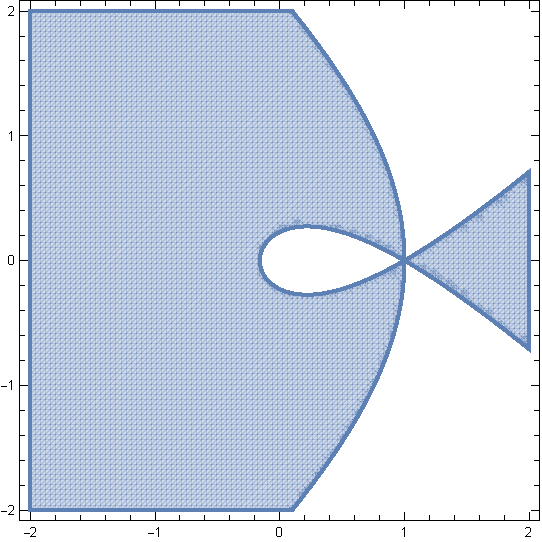
\includegraphics[height=.3\textwidth]{pictures/ReS_edge.pdf}
	\caption{The plot of the region $\operatorname{Re}S(z)-\operatorname{Re}S(1)>0$ for $X=2$.}
	\label{fig:ReS_edge}
\end{figure}

Thus, we have shown that under the rescaling, the GUE correlation kernel
$K_n(x,y)\ssp dy$ converges to a new kernel.
\begin{definition}
	\label{def:Airy_kernel}
	Define the \emph{Airy kernel} on $\mathbb{R}$ by
	\begin{equation*}
		K_{\mathrm{Ai}}(\xi,\eta)=\frac{1}{(2\pi i)^2}
		\int_{e^{-\frac{\pi i}{3}}\infty}^{e^{\frac{\pi i}{3}}\infty}dV
		\int_{e^{-\frac{2\pi i}{3}}\infty}^{e^{2\frac{\pi i}{3}}\infty}dU
		\ssp
		\frac{\exp\Bigl\{\frac{V^3-U^3}{3}+U\,\xi-V\,\eta\Bigr\}}{V-U}.
	\end{equation*}
	For another formula for the Airy kernel
	which does not involve integrals,
	see
	Problem~\ref{prob:airy}.
\end{definition}

\begin{proposition}
	\label{prop:edge}
	We have
	\begin{equation*}
		\lim_{n\to\infty}
		\frac{1}{n^{1/6}}K_n\Bigl(2\sqrt{n}+\frac{\xi}{n^{1/6}},\,2\sqrt{n}+\frac{\eta}{n^{1/6}}\Bigr)
		\to
		K_{\mathrm{Ai}}(\xi,\eta).
	\end{equation*}
	Consequently, the eigenvalue statistics at the edge of the spectrum converge to the Airy point process, in the sense of fine-dimensional distributions.
\end{proposition}

\subsection{Airy kernel, Tracy--Widom distribution, and convergence of the maximal
eigenvalue}

Let us make a few remarks on the asymptotic results of
\Cref{prop:bulk,prop:edge}.
First,
a rigorous justification of convergence
of contour integrals requires some estimates on the error terms
in the steepest descent analysis, but these
estimates are mild and not hard to obtain.

Second, the GUE has the maximal eigenvalue $\lambda_{max}$. It is reasonable
to assume that the Airy process also (almost surely) admits a maximal point
(usually denoted by $\mathfrak{a}_1$),
and that $\lambda_{max}$
converges to $\mathfrak{a}_1$ under appropriate rescaling:
\begin{equation}
	\label{eq:TW_GUE}
	\lim_{n\to\infty}n^{\frac{1}{6}}\bigl(\lambda_{max}-2\sqrt{n}\bigr)=\mathfrak{a}_1.
\end{equation}
This is indeed the case, but to show \eqref{eq:TW_GUE}, one needs to
show the convergence in distribution:
\begin{equation}
	\label{eq:TW_GUE_convergence}
	\lim_{n\to \infty}
	\mathbb{P}\Bigl(n^{1/6}(\lambda_{max}-2\sqrt{n})\le x\Bigr)
	\to
	\mathbb{P}(\mathfrak{a}_1\le x).
\end{equation}
Both events \eqref{eq:TW_GUE_convergence} are so-called
\emph{gap probabilities}, for example,
\begin{equation*}
	\operatorname{P}(\mathfrak{a}_1\le x)=
	\operatorname{P}(\textnormal{there are no eigenvalues in the interval $(x,\infty)$}),
\end{equation*}
which is expressed as
the Fredholm determinant
\begin{equation}
	\label{eq:gap-probability-Ai-Fredholm}
	\det\left( 1-K_{\mathrm{Ai}} \right)_{(x,\infty)}=
	1+\sum_{m=1}^{\infty}\frac{(-1)^m}{m!}
	\int_x^{\infty}dy_1\int_x^{\infty}dy_2\cdots
	\int_x^{\infty}dy_m
	\ssp
	\det\limits_{i,j=1}^m
	K_{\mathrm{Ai}}(y_i,y_j).
\end{equation}
Thus, to get \eqref{eq:TW_GUE_convergence}), one needs to show the convergence
of sums like this for the GUE kernel
to the corresponding sums for the Airy kernel. This is doable, but tedious.

Moreover, to get convergence in distribution of random variables,
one would also have to argue either \emph{tightness},
or independently show that
\eqref{eq:gap-probability-Ai-Fredholm} defines a
cumulative probability
distribution function in $x$:
\begin{equation}
	\label{eq:TW_GUE_cdf}
	F_2(x)=\det\left( 1-K_{\mathrm{Ai}} \right)_{(x,\infty)}.
\end{equation}
The distribution \eqref{eq:TW_GUE_cdf} is known as the \emph{GUE Tracy--Widom distribution}.
The subscript $2$ indicates that $\beta=2$. There are distributions
$F_\beta$ for all beta, most notably, the GOE and GSE distributions.
The classical distributions $F_1,F_2,F_4$ also appear as fluctuation distributions
in interacting particle systems, while other beta values do
not quite appear in the particle systems
domain.

More details
may be found in the original papers
\cite{tracy1993level},
\cite{Forrester1993},
\cite{tracy_widom1994level_airy}.




\appendix
\setcounter{section}{5}

\section{Problems (due 2025-03-19)}

\subsection{Different global positions}
\label{prob:different-global-positions}

Show that if in \eqref{eq:scaling_x-y} we take $X\ne Y$, then
$K_n(x,y)$ vanishes as $n\to+\infty$. Moreover,
establish that the decay is exponential in $n$.

\subsection{Sine kernel}
\label{prob:sine-kernel}

Compute the integral
\eqref{eq:K_n_bulk_single}.

\subsection{General bulk case}
\label{prob:imaginary-critical-points}

Perform the asymptotic analysis of the correlation
kernel as in \Cref{sub:imaginary-critical-points},
but in the general case $-2<X<2$.

\subsection{Discrete sine process}
\label{prob:discrete-sine-process}

Define the discrete sine kernel on $\mathbb{Z}$ by
\begin{equation*}
	K_{\mathrm{dsine}}(x,y)\coloneqq
	\begin{cases}
		\dfrac{\sin \rho(x-y)}{\pi (x-y)},&\qquad x\ne y,\\[10pt]
		\dfrac{\rho}{\pi},&\qquad x=y,
	\end{cases}
\end{equation*}
where $\rho\in[0,1]$ is the density parameter.

Let $\rho=1/2$.
Compute (numerically) the asymptotics of the two events under the discrete sine process:
\begin{equation*}
	\operatorname{\mathbb{P}}
	\Bigl(
		\underbrace{\circ \circ\ldots\circ}_{n\text{ times}}
		\underbrace{\bullet \bullet\ldots\bullet}_{n\text{ times}}
	\Bigr),\qquad
	\operatorname{\mathbb{P}}
	\Bigl(
		\underbrace{\circ\bullet\circ\bullet\ldots\circ\bullet}_{2n\text{ points}}
	\Bigr),\qquad
\end{equation*}
If the sine process was of independent random points (with the same density $1/2$),
both events
would have the same probability $2^{-2n}$.
Which event is more favored by the sine process?

\subsection{Large deviations}
\label{prob:large-deviation}

Let \(W_n\) be an \(n\times n\) Wigner real or Hermitian matrix with finite variance entries. Assume that the matrix is normalized so that the variance of each diagonal entry is 1.

\medskip

\textbf{Assumption \cite{BBP2005phase}.} \textit{If a Wigner matrix is normalized to have diagonal variance 1, then a rank 1 perturbation of magnitude $c>0$ is sufficient to shoot the maximum eigenvalue outside the support of the Wigner semicircle law. (For a simulation of this phenomenon, see \href{https://lpetrov.cc/simulations/2025-01-28-bbp-transition/}{here}.)}

\medskip

Consider the following large deviation event. For a fixed \(\eta>0\), let
\[
E_{n,\eta}\coloneqq \Bigl\{ \exists\, i\in\{1,\dots,n\} \text{ such that } W_{ii}\ge \eta \Bigr\}.
\]
Under the above assumption, if for some \(i\) the diagonal
entry \(W_{ii}\) is unusually large, it will push the
maximal eigenvalue of \(W_n\) outside the bulk.

\begin{enumerate}
	\item Assuming that the
		entries are Gaussian,
		\emph{lower bound} the probability of the event \(E_{n,\eta}\) for large \(n\).
	\item
		Assuming another tail behavior of the diagonal entries (exponential or
		power-law tails),
		use the limit theorems for maxima of independent random variables to generalize the
		\emph{lower bound} of $\operatorname{\mathbb{P}}(E_{n,\eta})$.
\end{enumerate}

\subsection{Airy kernel}
\label{prob:airy}

Define the Airy function by
\begin{equation*}
	Ai(\xi)\coloneqq
	\frac{1}{2\pi}\int_{-\infty}^\infty
	e^{i U^3/3+i\xi U} dU=
	\frac{1}{\pi}\int_0^\infty
	\cos\left( \frac{U^3}{3}+\xi U \right)\ssp dU.
\end{equation*}
This integral converges, but only conditionally. To improve convergence,
one should instead integrate
along a complex contour,
from $e^{\frac{5 \pi i}{6}}\infty$ to $0$ to
$e^{\frac{\pi i}{6}}\infty$.

Show that
\begin{equation*}
	K_{\mathrm{Ai}}(\xi,\eta)=
	\frac{Ai(\xi)\ssp Ai'(\eta)-Ai(\eta)\ssp Ai'(\xi)}{\xi-\eta}.
\end{equation*}
Note that this expression is parallel to the sine kernel,
\begin{equation*}
	\frac{\sin(x-y)}{\pi(x-y)}=\frac{\sin x\cos y-\cos x\sin y}{\pi(x-y)},\qquad
	\cos x=(\sin x)'.
\end{equation*}
These correlation kernels are called \emph{integrable}
\cite{its1990differential}.

Hint for the problem: observe that
\begin{equation*}
	\exp\left\{ -i z x+iwy \right\}=\frac{i}{x-y}\left( \frac{\partial}{\partial z}+
	\frac{\partial}{\partial w}\right)\exp\left\{ -i z x+iwy \right\},
\end{equation*}
and use integration by parts in $K_{\mathrm{Ai}}(\xi,\eta)$
from \Cref{def:Airy_kernel}.


\bibliographystyle{alpha}
\bibliography{bib}


\medskip

\textsc{L. Petrov, University of Virginia, Department of Mathematics, 141 Cabell Drive, Kerchof Hall, P.O. Box 400137, Charlottesville, VA 22904, USA}

E-mail: \texttt{lenia.petrov@gmail.com}


\end{document}
